% Kompilieren aus diesem Ordner: latexmk -pdf Versuchsdurchfuehrung.tex
% Alternativ: pdflatex Versuchsdurchfuehrung.tex (zweimal).
% Alle Fotos und Bildschirmaufnahmen liegen unter images/.
% Ablauf: notes.txt; Echozeiten werden aus dem gemessenen Peakabstand berechnet.
\documentclass[a4paper,11pt]{article}
\usepackage[T1]{fontenc}
\usepackage[utf8]{inputenc}
\usepackage[ngerman]{babel}
\usepackage{lmodern,microtype}
\usepackage[margin=19mm,top=19mm,bottom=19mm,headheight=14pt]{geometry}
\usepackage{graphicx,booktabs,tabularx,array,amsmath,amssymb}
\usepackage[export]{adjustbox}
\usepackage[table]{xcolor}
\usepackage{enumitem,parskip,fancyhdr,lastpage}
\usepackage[most]{tcolorbox}
\usepackage[font=small,labelfont=bf,labelsep=colon,skip=4pt,hypcap=false,justification=raggedright,singlelinecheck=false]{caption}
\usepackage[colorlinks=true,urlcolor=teal!65!black,linkcolor=teal!65!black]{hyperref}
\graphicspath{{images/}}
\definecolor{ink}{HTML}{15374A}
\definecolor{accent}{HTML}{087E8B}
\definecolor{pale}{HTML}{EEF5F7}
\hypersetup{pdftitle={Versuchsdurchführung: Magnetresonanztomographie},pdfauthor={},pdfsubject={Phantomaufbau, Scannerbedienung, Spektrum, Multi-Echo-Aufnahmen und DICOM-Export},pdfdisplaydoctitle=true}
\pagestyle{fancy}
\fancyhf{}
\fancyhead[L]{\small\sffamily\color{ink}MRT-PRAKTIKUM}
\fancyhead[R]{\small\sffamily Bedienung und Messablauf}
\fancyfoot[L]{\small\color{ink}Phantommessungen\enspace|\enspace Scan-Anleitung}
\fancyfoot[R]{\small\thepage\,/\,\pageref*{LastPage}}
\renewcommand{\headrulewidth}{0.4pt}
\setlength{\parindent}{0pt}
\setlength{\parskip}{5pt}
\setlength{\emergencystretch}{2em}
\setlist[enumerate]{leftmargin=6mm,itemsep=4pt,topsep=4pt}
\setlist[itemize]{leftmargin=5mm,itemsep=3pt,topsep=4pt}
\renewcommand{\arraystretch}{1.16}
\newcolumntype{Y}{>{\raggedright\arraybackslash}X}
\newcolumntype{P}[1]{>{\raggedright\arraybackslash}p{#1}}
\newcommand{\heading}[3]{\pdfbookmark[0]{#3}{#1}\label{#1}\vspace*{1mm}{\sffamily\bfseries\color{accent}\small #2\par}\vspace{1mm}{\sffamily\bfseries\color{ink}\LARGE #3\par}\vspace{2mm}}
\newcommand{\subhead}[1]{\par\vspace{2mm}{\sffamily\bfseries\color{ink}\large #1\par}\nopagebreak}
\newcommand{\ui}[1]{\textsf{\textbf{#1}}}
\newcommand{\seq}[1]{\texttt{#1}}
\newcommand{\ms}{\,\mathrm{ms}}
\newcommand{\blank}{\rule{20mm}{0.35pt}}
\newtcolorbox{note}{colback=pale,colframe=accent!45,boxrule=.5pt,arc=1mm,left=3mm,right=3mm,top=2mm,bottom=2mm,before skip=6pt,after skip=6pt}
% Relative Beschnitte sind unabhängig von den DPI. Originalbilder bleiben unverändert.
\newcommand{\bild}[3][]{\par\noindent\begin{minipage}{\linewidth}\centering\adjincludegraphics[width=\linewidth,#1]{#2}\captionof{figure}{#3}\end{minipage}\par}

\begin{document}

% Titelbereich nach dem Versuchsskript "Bildgebende Verfahren -
% Magnetresonanztomographie". Logo und MRT-Foto sind unveränderte
% Bildressourcen aus der ersten PDF-Seite; die Kennzeichnung ist angepasst.
% Das Deckblatt ist unnummeriert. Die Scan-Anleitung beginnt danach bei 1.
\hypersetup{pageanchor=false}
\begin{titlepage}
\thispagestyle{empty}
\pdfbookmark[0]{Versuchsdurchführung}{deckblatt}
\definecolor{deckblattblau}{HTML}{00549F}
\definecolor{deckblattgrau}{HTML}{666666}
\begin{tikzpicture}[remember picture,overlay]
  \node[anchor=north west,inner sep=0pt]
    at ([xshift=64.03mm,yshift=-31.06mm]current page.north west)
    {
\includegraphics[width=125.94mm]{deckblatt_logo.png}};

  \node[anchor=north west,inner sep=0pt,text=deckblattgrau,
        font={\fontfamily{phv}\fontsize{12bp}{14bp}\selectfont}]
    at ([xshift=25.4mm,yshift=-75.20mm]current page.north west)
    {Praktikum Medizintechnik - Versuchsdurchführung};

  \node[anchor=north west,inner sep=0pt,text=deckblattblau,
        font={\fontfamily{phv}\fontsize{26bp}{31bp}\selectfont\bfseries}]
    at ([xshift=25.4mm,yshift=-83.40mm]current page.north west)
    {Magnetresonanztomographie};

  \node[anchor=north west,inner sep=0pt,align=left,text=deckblattblau,
        font={\fontfamily{phv}\fontsize{23bp}{30.415bp}\selectfont}]
    at ([xshift=25.4mm,yshift=-95.40mm]current page.north west)
    {Fett-Wasser-Trennung mit der Dixon-\\Methode am 1.5 Tesla MRT};

  \node[anchor=north west,inner sep=0pt]
    at ([xshift=25.93mm,yshift=-121.28mm]current page.north west)
    {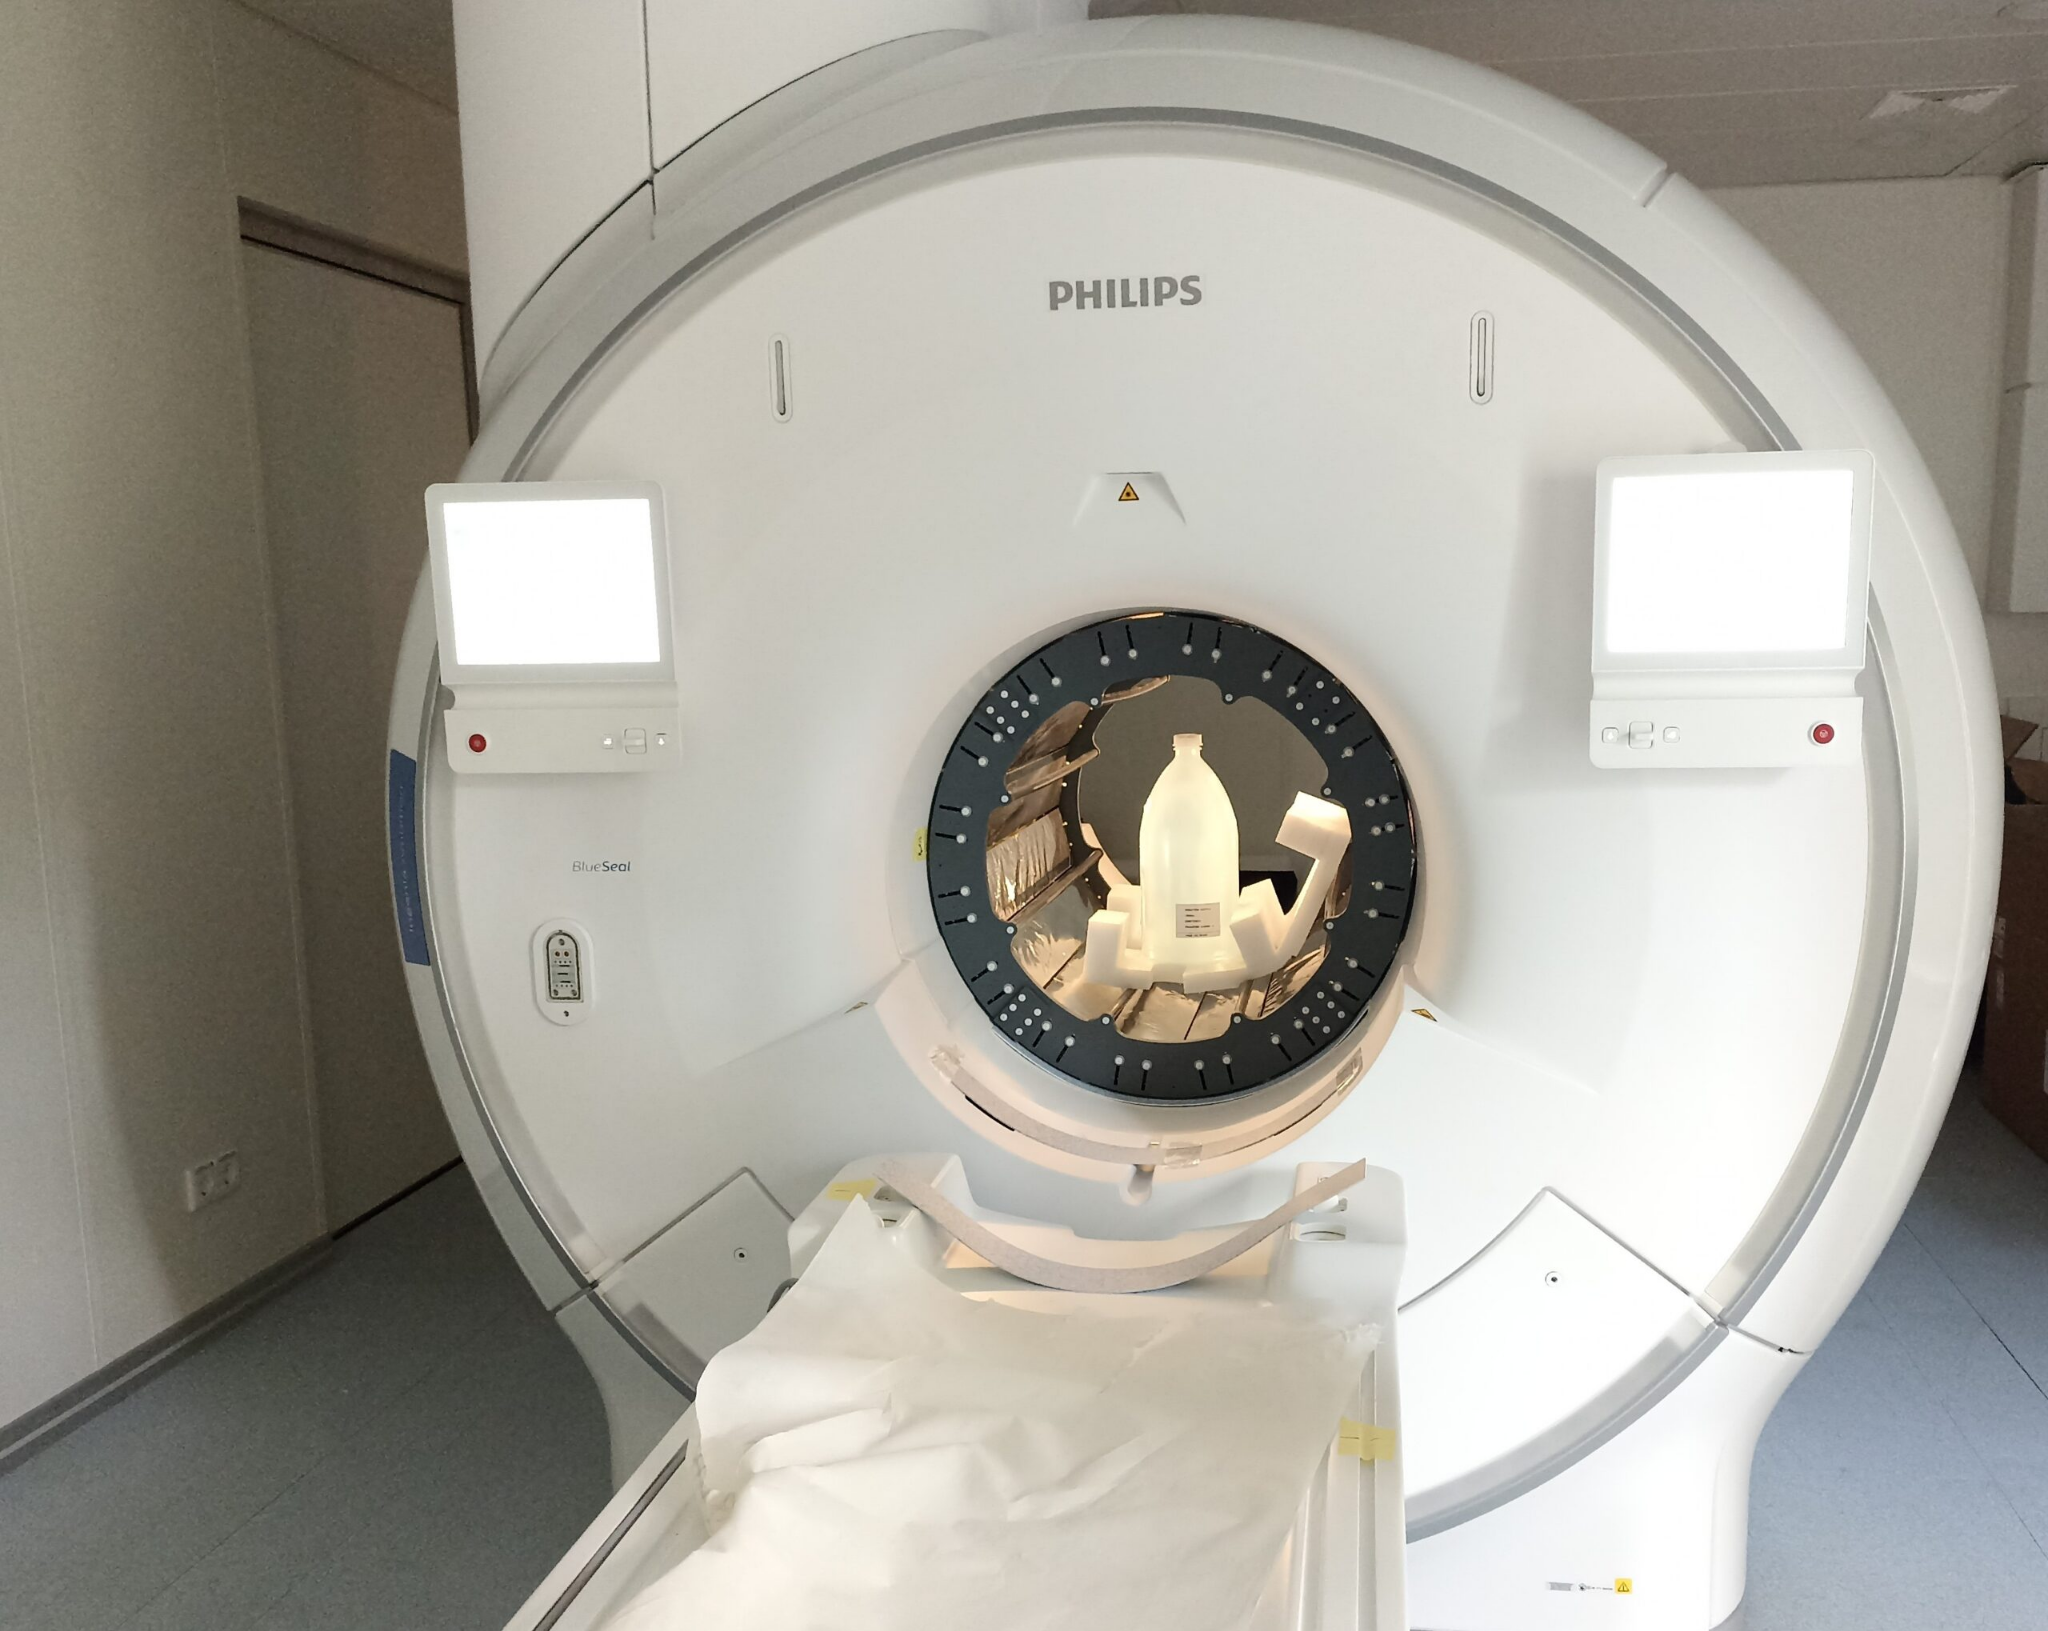
\includegraphics[width=88.64mm]{deckblatt_mrt.png}};
\end{tikzpicture}
\null
\end{titlepage}
\hypersetup{pageanchor=true}


\heading{registrierung}{01 / START UND REGISTRIERUNG}{MRT-Scananleitung}
Diese Anleitung führt Sie vom Einrichten eines Phantomversuchs bis zum Export der Messdaten. Sie üben die Schichtplanung, nehmen ein T1- und ein T2-gewichtetes Referenzbild auf, vergleichen damit zwei Flipwinkel, bestimmen den Wasser-Fett-Frequenzabstand und nehmen zwei bzw.\ drei Echozeiten zuerst einzeln und dann gemeinsam in einer Messung auf. Die Dixon-Auswertung im Notebook vergleicht \textbf{eine gemeinsame Schichtebene}; die $B_0$-Auswertung ist optional.

\begin{note}
\textbf{Messfolge:} Phantom registrieren $\rightarrow$ Spule und Objekt aufbauen $\rightarrow$ Position einmessen $\rightarrow$ Survey aufnehmen $\rightarrow$ T1W- und T2W-Referenzbild aufnehmen $\rightarrow$ zwei Flipwinkel vergleichen $\rightarrow$ Spektrum messen $\rightarrow$ zwei und drei Echos einzeln und kombiniert aufnehmen $\rightarrow$ Objektvarianten vergleichen $\rightarrow$ DICOM exportieren.
\end{note}

\subhead{Für jede Gruppe eine eigene Untersuchung anlegen}
\begin{enumerate}
\item Öffnen Sie nach dem Softwarestart \ui{Patients $\rightarrow$ New Examination\ldots} oder drücken Sie \ui{F2}.
\item Tragen Sie unter \ui{Patient name} und \ui{Registration ID} eine eindeutige Gruppenkennung ein, z.\,B. \texttt{Praktikum1}. Verwenden Sie die mit der Betreuung vereinbarten Angaben für weitere Pflichtfelder.
\item Wählen Sie unter \ui{Gender} den Typ \ui{Phantom} und tragen Sie unter \ui{Patient weight} \textbf{5\,kg} ein.
\item Speichern und öffnen Sie die Untersuchung mit \ui{Confirm and Proceed}. Richten Sie danach den Versuchsaufbau auf dem Tisch ein.
\end{enumerate}

\noindent\begin{minipage}[t]{.35\linewidth}\vspace{0pt}
\bild[trim={0\width} {.77\height} {.835\width} {0\height},clip]{NEW_PATIENT_1.png}{Neue Untersuchung im Menü \ui{Patients}.}
\end{minipage}\hfill
\begin{minipage}[t]{.61\linewidth}\vspace{0pt}
\bild[trim={.105\width} {.63\height} {.63\width} {.167\height},clip]{NEW_PATIENT_2.png}{Gruppenkennung, \ui{Phantom} und \textbf{5\,kg} im Registrierungsdialog.}
\end{minipage}

\begin{note}
\textbf{Aufbau mit der Betreuung:} Lassen Sie Spulenanschluss, Tischbewegungen und Messfreigabe vor Ort begleiten. Für den Versuch mit Metallknopf verwenden Sie ausschließlich das bereitgestellte Versuchsobjekt nach Freigabe durch die Betreuung. Mitgebrachte Objekte werden vor dem Einbringen geprüft.
\end{note}

\newpage
\heading{aufbau}{02 / VERSUCHSAUFBAU}{Material und Kopfspule vorbereiten}
Diese Materialien stehen für den Versuch bereit. Das Foto dient nur der Materialübersicht.

\bild[trim={0\width} {.25\height} {0\width} {.355\height},clip]{mr_needed_material.JPG}{Materialübersicht; die Zuordnung folgt von links nach rechts.}

\begin{tabularx}{\linewidth}{@{}P{8mm}P{54mm}Y@{}}
\toprule
\textbf{Nr.} & \textbf{Material} & \textbf{Verwendung} \\
\midrule
1 & Wasserphantom & Referenzobjekt mit Wasser. \\
2 & Sandsäcke & Objekt innerhalb der Spule gegen Verrutschen sichern. \\
3 & Wasser-/Ölflasche & Zwei Flüssigkeitsbereiche für Spektrum und Dixon. \\
4 & Kittel mit eisenhaltigem Knopf & Bereitgestelltes Störobjekt für den Artefaktvergleich. \\
5 & Kopfspulen-Oberteil & Spule nach der Lagerung schließen. \\
6 & Kopfspulen-Unterteil & Aufnahme und Lagerung des Messobjekts. \\
\bottomrule
\end{tabularx}

\subhead{Kopfspule anschließen und Objekt lagern}
\noindent\begin{minipage}[t]{.47\linewidth}\vspace{0pt}
\bild[trim={.10\width} {.11\height} {.24\width} {.12\height},clip]{installed_headcoil.JPG}{Aufgesetztes Oberteil der Kopfspule am Kopfende des Tisches.}
\end{minipage}\hfill
\begin{minipage}[t]{.49\linewidth}\vspace{0pt}
\begin{enumerate}
\item Platzieren Sie das Unterteil am Kopfende des Tisches. Schließen Sie die Kopfspule am \textbf{oberen Anschluss an der Kopfseite} an.
\item Legen Sie das gewählte Objekt in die Spule. Sichern Sie es bei Bedarf mit Sandsäcken.
\item Setzen Sie das Oberteil auf und lassen Sie Sitz und Anschluss prüfen.
\item Lassen Sie Wasser und Öl zur Ruhe kommen. Behalten Sie die Lagerung zwischen Vergleichsaufnahmen bei.
\end{enumerate}
\end{minipage}

\newpage
\heading{position}{03 / OBJEKTPOSITION}{Die Objektmitte einmessen}
Der Scanner benötigt die Position des Objekts auf dem Tisch. Verwenden Sie dafür die Bedienelemente unter dem seitlichen Display.

\noindent\begin{minipage}[t]{.49\linewidth}\vspace{0pt}
% EXIF-Orientierung 3: pdfLaTeX benötigt eine explizite Drehung um 180 Grad.
\bild[angle=180,trim={.18\width} {.08\height} {.20\width} {.05\height},clip]{mr_display.JPG}{Seitliches Display mit den Tasten unterhalb des Bildschirms: Laser links, Kippschalter mittig, Bestätigung rechts.}
\end{minipage}\hfill
\begin{minipage}[t]{.47\linewidth}\vspace{0pt}
\begin{enumerate}
\item Aktivieren Sie den Positionierlaser mit der \textbf{linken Taste neben dem Kippschalter} (Lampensymbol). Auf dem Tisch erscheint eine rote Laserlinie.
\item Fahren Sie den Tisch mit dem \textbf{Kippschalter} so weit nach vorne, bis die Laserlinie die \textbf{Mitte des Objekts in der Kopfspule} trifft.
\item Bestätigen Sie die Position mit der \textbf{rechten Taste} (Tischsymbol). Diese leuchtet anschließend grün.
\item Lassen Sie die weitere Tischpositionierung und die Freigabe zum Messen von der Betreuung begleiten.
\end{enumerate}
\end{minipage}

\subhead{Orientierung im Scanfenster}
\noindent\begin{minipage}[t]{.52\linewidth}\vspace{0pt}
\bild{START_SCREEN.png}{Scanfenster vor dem Laden einer Sequenz.}
\end{minipage}\hfill
\begin{minipage}[t]{.44\linewidth}\vspace{0pt}
\begin{itemize}
\item \textbf{Links:} Sequenzliste der aktuellen Untersuchung und Messstatus.
\item \textbf{Rechts oben:} Vorschau, Planungsansichten und geladene Bilder.
\item \textbf{Unten:} \ui{ExamCards} als Sequenzbibliothek bzw. Parameter der geöffneten Sequenz.
\item \textbf{Links unten:} \ui{Start Scan} zum Starten der bestätigten Sequenz.
\end{itemize}
\end{minipage}

\begin{note}
\textbf{Nächster Schritt: Survey.} Die eingemessene Tischposition ersetzt die Bildplanung nicht. Nehmen Sie zunächst eine Übersicht auf und planen Sie darauf die folgenden Messungen.
\end{note}

\newpage
\heading{survey}{04 / ERSTE MESSUNG}{Survey laden, bestätigen und starten}
\begin{enumerate}
\item Öffnen Sie unten die \ui{ExamCards}. Die Praktikumssequenzen liegen unter \ui{Hospital $\rightarrow$ LfB $\rightarrow$ MR-Praktikum}.
\item Ziehen Sie zuerst \seq{Survey (CS Sequenzen)} mit gedrückter Maustaste aus der Bibliothek in die \textbf{linke Sequenzliste}.
\item Öffnen Sie den Eintrag per Doppelklick. Prüfen Sie die Einstellungen und bestätigen Sie mit dem grünen \ui{Accept}. \textbf{Erst danach} starten Sie links unten mit \ui{Start Scan}.
\item Warten Sie das Messende ab. Die laufende Aufnahme zeigt einen Fortschrittsbalken; eine fertige Sequenz ist blau hinterlegt und trägt ein Häkchen. Öffnen Sie das Ergebnis per Doppelklick.
\end{enumerate}

\noindent\begin{minipage}[t]{.48\linewidth}\vspace{0pt}
\bild[trim={.21\width} {.25\height} {.40\width} {.53\height},clip]{LOAD_SEQUENCE_1.png}{Bibliothek im Reiter \ui{Hospital}: Survey und weitere Praktikumssequenzen.}
\end{minipage}\hfill
\begin{minipage}[t]{.48\linewidth}\vspace{0pt}
\bild[trim={0\width} {.41\height} {.39\width} {.155\height},clip]{LOAD_SEQUENCE_2.png}{Survey in der linken Liste; grünes \ui{Accept} zum Übernehmen der Parameter.}
\end{minipage}

\noindent\begin{minipage}[t]{.25\linewidth}\vspace{0pt}
\bild[trim={0\width} {0\height} {.793\width} {.87\height},clip]{SCAN_RUNNING.png}{Während der Messung: Fortschritt und Restzeit links unten.}
\end{minipage}\hfill
\begin{minipage}[t]{.71\linewidth}\vspace{0pt}
\bild[trim={0\width} {.47\height} {0\width} {.045\height},clip]{SCAN_RESULT.png}{Abgeschlossener Survey mit Häkchen und drei Übersichtsansichten des Objekts.}
\end{minipage}

\begin{note}
\textbf{Planungsgrundlage:} Der Survey liefert ein grobes Bild von Lage und Ausdehnung des Objekts. Alle weiteren Aufnahmen werden auf dieser Übersicht geplant; als erste davon ein T2- und ein T1-gewichtetes Referenzbild (Abschnitt \hyperref[referenz]{07}). Nach einem Objektwechsel nehmen Sie einen neuen Survey auf.
\end{note}

\newpage
\heading{viewer}{05 / BILDBETRACHTER}{Aufnahmen im Review ansehen und vergleichen}
Jede abgeschlossene Sequenz öffnen Sie per Doppelklick in der linken Liste. Die Oberfläche wechselt dann von \ui{Plan} nach \ui{Review}; beide Schaltflächen stehen rechts neben den Patientendaten. Jede geöffnete Serie erscheint als eigenes Fenster \ui{ImageView}. Mit \ui{Plan} kehren Sie zur Sequenzplanung zurück, ohne die Bildfenster zu verlieren.

\bild[trim={0\width} {.47\height} {0\width} {.045\height},clip]{REVIEW_IMAGEVIEW.png}{Review mit zwei Bildfenstern derselben Serie: links die Phase (\texttt{/P}), rechts die Magnitude (\texttt{/M}) von Schicht 3 von 5.}

\subhead{Bildkopf lesen}
Links oben in jedem Bild stehen die wichtigsten Kennungen. Prüfen Sie sie bei jedem Vergleich, bevor Sie Signalunterschiede interpretieren.

\begin{tabularx}{\linewidth}{@{}P{34mm}Y@{}}
\toprule
\textbf{Eintrag} & \textbf{Bedeutung} \\
\midrule
\texttt{Sc 4,1} & Scan 4 der Untersuchung, erste Wiederholung; entspricht der Nummer in der linken Liste. \\
\texttt{Sl 3/5} & Schicht 3 von 5 des Stapels. Vergleichen Sie Echos immer auf derselben Schichtnummer. \\
\texttt{FFE /M} & Sequenztyp und Bildkomponente: \texttt{/M} Magnitude, \texttt{/P} Phase. Beide Komponenten liegen als getrennte Bilder vor. \\
\texttt{H F R L A P} & Patientenachsen am Bildrand: Kopf/Fuß, rechts/links, anterior/posterior. \\
\bottomrule
\end{tabularx}

\subhead{Im Bild navigieren}
\begin{itemize}
\item \textbf{Schichten blättern:} Fahren Sie mit der Maus über das Bild und drehen Sie das Mausrad. Die Schichtnummer \texttt{Sl} im Bildkopf zählt mit.
\item \textbf{Werkzeugleiste:} Oberhalb jedes Bildfensters finden Sie Symbole für Bildlayout, Cine-Wiedergabe, Beschriftung, Messlineal, Fensterung (Helligkeit/Kontrast) und das Verschieben des Bildausschnitts sowie die Menüs \ui{Viewing}, \ui{Printing} und \ui{More}. Ein Tooltip nennt das Werkzeug und die zugehörige Maustaste.
\item \textbf{Fensterung:} Mit dem Kontrastwerkzeug ziehen Sie mit gedrückter Maustaste im Bild: waagerecht ändert die Fensterbreite (Kontrast), senkrecht die Fenstermitte (Helligkeit). Die Fensterung ändert nur die Anzeige, nicht die gespeicherten Werte.
\item \textbf{Mehrere Fenster:} Mit den Layout-Symbolen ganz links in der oberen Leiste teilen Sie den Bereich in mehrere Bildfenster. Öffnen Sie die zu vergleichenden Serien nacheinander per Doppelklick und stellen Sie in allen Fenstern dieselbe Schichtnummer ein.
\item \textbf{Bildfenster schließen:} Über das Kreuz rechts in der Titelzeile des jeweiligen \ui{ImageView}.
\end{itemize}

\bild[trim={.21\width} {.883\height} {.396\width} {.048\height},clip]{REVIEW_IMAGEVIEW.png}{Werkzeugleiste eines Bildfensters mit Serienname, Layout-, Cine-, Beschriftungs-, Mess- und Fensterungswerkzeugen.}

\begin{note}
\textbf{Phasenbilder richtig lesen:} Ein Phasenbild zeigt Winkel von $-\pi$ bis $\pi$ als Grauwerte. Scharfe Hell-Dunkel-Sprünge im Objekt sind Phasenumbrüche und keine Strukturen. Im signalarmen Hintergrund ist die Phase Rauschen. Für den Echovergleich nutzen Sie zunächst die Magnituden; die Phasen werden im Notebook ausgewertet.
\end{note}

{\small\textbf{AutoView während der Messung:} Im Reiter \ui{AutoView} rechts unten im Planungsfenster erscheint das jeweils zuletzt rekonstruierte Bild schon während der laufenden Aufnahme. So erkennen Sie früh, ob Lage und Signal stimmen.}

\heading{parameter}{06 / PARAMETER EINSTELLEN}{Sequenzparameter ändern und Echos verteilen}
Ein Doppelklick auf eine noch nicht gemessene Sequenz öffnet sie im Modus \ui{Plan}. Oben zeigen drei Planungsansichten den Schichtstapel (orange) mit den nummerierten Schichten (rot); unten liegt der Parameterbereich mit den Reitern \ui{Summary}, \ui{Geometry}, \ui{Contrast}, \ui{Motion}, \ui{Dyn/Ang}, \ui{Postproc}, \ui{Offc/Ang}, \ui{Coils} und \ui{Conflicts}. Rechts daneben zeigt der Reiter \ui{Info} die aus den Einstellungen berechneten Werte.

\subhead{So ändern Sie einen Wert}
\begin{enumerate}
\item Wählen Sie den Reiter, z.\,B. \ui{Contrast}, und klicken Sie die Zeile an. Die gewählte Zeile wird blau hinterlegt.
\item Die rechte Spalte enthält entweder eine Auswahlliste (z.\,B. \ui{shortest}, \ui{user defined}, \ui{default}) oder ein Zahlenfeld. Bei \ui{user defined} erscheint direkt darunter eine eingerückte Zeile mit der Einheit, hier \ui{(ms)}, in die Sie den Wert eintragen.
\item Abhängige Werte passen sich sofort an. Unzulässige Kombinationen meldet der Reiter \ui{Conflicts}; die Messung lässt sich erst nach dem Beheben starten.
\item Kontrollieren Sie im Reiter \ui{Info} die tatsächlichen Werte: \ui{Act.\ TR/TE1/delta TE} zeigt das umgesetzte TR, die erste Echozeit und den Echoabstand; \ui{Min.\ TR/TE1/delta TE} nennt die am Scanner kleinsten erreichbaren Werte. Dort stehen auch Messdauer, Matrix und Voxelgröße.
\item Übernehmen Sie mit dem grünen \ui{Accept} oder verwerfen Sie mit \ui{Cancel}. Die Kopfzeile über den Reitern zeigt nach dem Übernehmen Messdauer, Voxel, relatives SNR, TE und TR. Starten Sie danach mit \ui{Start Scan}.
\end{enumerate}

\bild[trim={.21\width} {.42\height} {.396\width} {.533\height},clip,width=.8\linewidth]{PLAN_TRIPLE_ECHO.png}{Kopfzeile der geöffneten Sequenz mit Messdauer, Voxel, relativem SNR, TE, TR und dem grünen \ui{Accept}.}

\subhead{Echoanzahl, erste Echozeit und Echoabstand}
Bei den Multi-Echo-FFE-Sequenzen dieses Praktikums geben Sie die Echozeiten nicht einzeln ein. Im Reiter \ui{Contrast} bestimmen drei Zeilen die Verteilung der Echos:

\begin{tabularx}{\linewidth}{@{}P{36mm}P{30mm}Y@{}}
\toprule
\textbf{Zeile} & \textbf{Beispielwert} & \textbf{Bedeutung} \\
\midrule
\ui{Echoes} & 3 & Anzahl der Echos je Anregung. Jedes Echo liefert ein eigenes Bild. \\
\ui{TE first} & user defined, 9.2 & Echozeit $TE_1$ des ersten Echos in ms. \\
\ui{echospacing} & user defined, 6.9 & Abstand $\Delta TE$ zwischen zwei aufeinanderfolgenden Echos in ms. \\
\ui{flyback} & no & Auslesemodus; die Voreinstellung bleibt. \\
\bottomrule
\end{tabularx}

Die Echos liegen damit \textbf{äquidistant}:
\[
TE_k = TE_1 + (k-1)\,\Delta TE,\qquad k=1,\dots,N .
\]
Mit den Beispielwerten ergeben sich $TE_1=9.2\ms$, $TE_2=16.1\ms$ und $TE_3=23.0\ms$; der Reiter \ui{Info} bestätigt das als \ui{Act.\ TR/TE1/delta TE = 200 / 9.2 / 6.9}. Die tatsächlichen Werte stehen später auch in den DICOM-Metadaten.

\noindent\begin{minipage}[t]{.44\linewidth}\vspace{0pt}
\bild[trim={.211\width} {.033\height} {.601\width} {.583\height},clip]{PLAN_TRIPLE_ECHO.png}{Reiter \ui{Contrast} mit \ui{Echoes}, \ui{TE first} und \ui{echospacing}.}
\end{minipage}\hfill
\begin{minipage}[t]{.52\linewidth}\vspace{0pt}
\bild[trim={.404\width} {.062\height} {.396\width} {.607\height},clip]{PLAN_TRIPLE_ECHO.png}{Reiter \ui{Info}: tatsächliche und minimal erreichbare Werte für TR, TE1 und Echoabstand.}
\end{minipage}

\begin{itemize}
\item \textbf{Zwei Echos:} $TE_1$ und $TE_2=TE_1+\Delta TE$ sind frei wählbar. Tragen Sie die kleinere Zeit als \ui{TE first} und die Differenz als \ui{echospacing} ein.
\item \textbf{Drei Echos:} Das mittlere Echo liegt automatisch in der Mitte, $TE_3-TE_1=2\,\Delta TE$. Für die $B_0$-Aufgabe planen Sie deshalb den \textbf{Echoabstand}, nicht die äußeren Zeiten einzeln.
\item \textbf{Grenzen:} \ui{TE first} und \ui{echospacing} müssen über den Werten in \ui{Min.\ TR/TE1/delta TE} liegen; im Beispiel sind das $3.7\ms$ und $3.2\ms$. Der kleinste Echoabstand hängt von Auflösung und Bandbreite (\ui{Act.\ WFS / BW}) ab. Ein spätes letztes Echo kann ein längeres TR erzwingen.
\item \textbf{Bildkomponenten:} Ob je Echo Magnitude, Phase oder beides gespeichert wird, stellen Sie unter \ui{Postproc} ein. Für die $B_0$-Karte benötigen Sie beide Komponenten.
\end{itemize}

\begin{note}
\textbf{Beispielwerte sind keine Vorgabe.} Die gezeigten $9.2\ms$ und $6.9\ms$ stammen aus der vorbereiteten ExamCard. Berechnen Sie Ihre eigenen Werte aus dem im Spektrum gemessenen Frequenzabstand (Abschnitt \hyperref[spektrum]{09}) und dokumentieren Sie jede Änderung.
\end{note}

\newpage
\heading{referenz}{07 / REFERENZBILDER}{T1W- und T2W-Referenzbild aufnehmen}
Bevor Sie den Kontrast selbst verändern, nehmen Sie zwei Referenzbilder mit vorgefertigten Sequenzen aus den Vorlagen auf: ein \textbf{T2-gewichtetes} und ein \textbf{T1-gewichtetes} Bild derselben Ebene. Dabei üben Sie auch die Schichtplanung. Beide Bilder dienen im folgenden Kapitel als Vergleich für die Flipwinkelaufnahmen.

\subhead{T2W-Referenzbild: Schichten planen}
\begin{enumerate}
\item Öffnen Sie die \ui{ExamCards} und wechseln Sie zu den Vorlagen im Reiter \ui{Philips}. Ziehen Sie eine T2-gewichtete TSE-Sequenz, z.\,B. \seq{T2W\_TSE}, in die linke Sequenzliste und öffnen Sie sie per Doppelklick.
\item Unter \ui{Summary} stehen Bildfeld (\emph{Field of View}, FOV), Voxel und Schichtanzahl, unter \ui{Geometry} die Details. Verschieben und drehen Sie den Schichtstapel in den drei Planungsansichten auf dem Survey; die \textbf{roten Linien und Zahlen} zeigen die geplanten Schichten.
\item Variieren Sie Bildfeld, Position, Orientierung und Schichtanzahl, bis das Objekt vollständig im Bildfeld liegt. Wählen Sie eine Ebene durch \textbf{Wasser, Öl und den Übergang} und beachten Sie die Messdauer in der Kopfzeile.
\item Bestätigen Sie mit \ui{Accept}, starten Sie mit \ui{Start Scan} und öffnen Sie das Ergebnis im \ui{Review} (Abschnitt \hyperref[viewer]{05}). Notieren Sie Position, Orientierung, FOV und Schichtdicke; diese Geometrie übernehmen Sie für alle folgenden Aufnahmen.
\end{enumerate}

\bild[trim={.21\width} {.47\height} {0\width} {.045\height},clip,width=.76\linewidth]{SEQUENCE_FOV_PLANNING.png}{Schichtplanung der Vorlage \seq{T2W\_TSE} auf dem Survey; rote Linien markieren die Schichten. Die T2W-TSE-Werte sind keine Vorgabe für die FFE-Messungen.}

\subhead{T1W-Referenzbild}
\begin{enumerate}
\item Ziehen Sie aus den Vorlagen im Reiter \ui{Philips} eine T1-gewichtete Sequenz, z.\,B. \seq{T1W\_TSE}, in die linke Sequenzliste und öffnen Sie sie per Doppelklick.
\item Übernehmen Sie Position, Orientierung, Schichtdicke und FOV der T2W-Referenz, damit beide Bilder dieselbe Ebene zeigen.
\item Bestätigen Sie mit \ui{Accept}, starten Sie mit \ui{Start Scan} und öffnen Sie das Ergebnis im \ui{Review}.
\item Stellen Sie beide Referenzbilder in zwei Bildfenstern auf derselben Schichtnummer nebeneinander. Wie erscheinen Wasser und Öl im T1W- und im T2W-Bild? Halten Sie Ihre Beobachtung in der Tabelle im nächsten Kapitel fest.
\end{enumerate}

\begin{note}
\textbf{Für beide Referenzbilder notieren:} Sequenzname, TR, TE und Flipwinkel aus der Kopfzeile bzw.\ dem Reiter \ui{Info}. Erst damit lassen sich die Kontraste später den Sequenzparametern zuordnen.
\end{note}

\newpage
\heading{flipwinkel}{08 / FLIPWINKEL}{Zwei Flipwinkel aufnehmen und mit den Referenzen vergleichen}
Der Flipwinkel bestimmt, wie weit die Magnetisierung bei jeder Anregung ausgelenkt wird. Bei einer Gradientenechosequenz mit kurzem TR verändert er damit, wie stark das Bild T1-gewichtet ist.
\begin{enumerate}
\item Laden Sie aus \ui{Hospital $\rightarrow$ LfB $\rightarrow$ MR-Praktikum} ein vorbereitetes FFE-Protokoll, z.\,B. \seq{T1W\_FFE IP}. Übernehmen Sie Position, Orientierung, Schichtdicke und FOV der Referenzbilder.
\item Nehmen Sie \textbf{zwei Bilder mit deutlich verschiedenen Flipwinkeln} auf, z.\,B. mit dem voreingestellten Winkel und mit einem deutlich größeren. Den Winkel ändern Sie im Reiter \ui{Contrast} in der Zeile \ui{Flip angle} (Bedienung in Abschnitt \hyperref[parameter]{06}). Halten Sie alle übrigen Parameter, insbesondere TR und TE, für beide Aufnahmen konstant.
\item Bestätigen Sie jede Einstellung mit \ui{Accept} und starten Sie mit \ui{Start Scan}.
\item Vergleichen Sie beide Flipwinkelbilder untereinander und mit der \textbf{T1W- und der T2W-Referenz} auf derselben Schichtnummer. Welchem Referenzkontrast ähnelt welches Bild? Wie verändern sich Signal und Kontrast von Wasser und Öl mit dem Flipwinkel?
\end{enumerate}

\subhead{Kontraste vergleichen}
\begin{tabularx}{\linewidth}{@{}P{34mm}P{30mm}P{24mm}Y Y@{}}
\toprule
\textbf{Aufnahme} & \textbf{Sequenz} & \textbf{Flipwinkel [$^\circ$]} & \textbf{Signal Wasser} & \textbf{Signal Öl} \\
\midrule
T2W-Referenz & \hrulefill & \hrulefill & \hrulefill & \hrulefill \\
T1W-Referenz & \hrulefill & \hrulefill & \hrulefill & \hrulefill \\
Flipwinkel 1 & \hrulefill & \hrulefill & \hrulefill & \hrulefill \\
Flipwinkel 2 & \hrulefill & \hrulefill & \hrulefill & \hrulefill \\
\bottomrule
\end{tabularx}

\begin{note}
\textbf{Für die folgenden Echovergleiche:} Behalten Sie Position, Orientierung, Schichtdicke, FOV und Matrix bei und stellen Sie nach dem Flipwinkelversuch wieder den für die Multi-Echo-Messung vorgesehenen Winkel ein. Behalten Sie den vorbereiteten Aufnahmemodus bei: Eine gemeinsame Auswerteebene kann auch aus einem \textbf{3D-Schichtstapel} stammen.
\end{note}

\newpage
\heading{spektrum}{09 / FREQUENZBESTIMMUNG}{Wasser- und Fettpeak im Spektrum finden}
\begin{enumerate}
\item Laden Sie \seq{T1W\_FFE spectrum}, übernehmen Sie die geplante Geometrie und starten Sie nach \ui{Accept} die Messung.
\item Es öffnet sich die \ui{Monitoring Console} zur interaktiven $f_0$-Bestimmung. Lesen Sie die Resonanzfrequenz (Larmorfrequenz) in der Kopfzeile und die Frequenzpositionen der Peaks auf der horizontalen Achse ab.
\item Messen Sie zunächst die \textbf{Wasserflasche} als Referenz und anschließend die \textbf{Wasser-/Ölflasche}. Nach dem Umbau erneut einmessen und einen Survey aufnehmen. Ordnen Sie den Wasserpeak durch den Vergleich zu und suchen Sie im Gemisch den Fett-/Ölpeak.
\item Notieren Sie die beiden Peakpositionen und den \textbf{Betrag ihres Frequenzabstands}. Beachten Sie die Richtung der beschrifteten Frequenzachse. Schließen Sie die interaktive Bestimmung nach Rücksprache mit der Betreuung mit \ui{Proceed} ab.
\end{enumerate}

\noindent\begin{minipage}{.68\linewidth}
\bild[trim={.003\width} {.417\height} {.47\width} {.083\height},clip]{SEQUENCE_SPECTRUM.png}{Spektrum mit Resonanzfrequenz und relativer Frequenzachse in Hz.}
\end{minipage}\hfill
\begin{minipage}{.28\linewidth}
{\small Die automatische Meldung \texttt{no fat detected} ersetzt die eigene Peakzuordnung nicht. Vergleichen Sie Wasserreferenz und Gemisch.}
\end{minipage}

\newpage
\subhead{Aus dem Peakabstand die Echozeiten vorbereiten}
Bezeichnen Sie die abgelesenen relativen Peakpositionen mit $f_\mathrm{W}$ und $f_\mathrm{F}$. Die chemische Phasendifferenz durchläuft in der Zeit $T_\mathrm{cs}$ eine volle Umdrehung:
\[
|\Delta f_\mathrm{cs}|=|f_\mathrm{W}-f_\mathrm{F}|,
\qquad T_\mathrm{cs}=\frac{1}{|\Delta f_\mathrm{cs}|}.
\]
Setzen Sie den Frequenzabstand in Hz ein; dann erhalten Sie $T_\mathrm{cs}$ in Sekunden. Für die TE-Eingabe rechnen Sie in Millisekunden um.

\begin{note}
\textbf{Mit der Vorbereitung vergleichen:} Vergleichen Sie den gemessenen Peakabstand $|\Delta f_\mathrm{cs}|$ mit dem Wert, den Sie im Vorfeld aus der chemischen Verschiebung von $3.5\,\mathrm{ppm}$ für $1.5\,\mathrm{T}$ berechnet haben (Versuchsskript). \textbf{Warum unterscheidet sich der im Vorfeld berechnete Wert vom tatsächlich gemessenen Frequenzabstand?}
\par\vspace{1mm} Berechnet: \blank\ Hz \hfill Gemessen: \blank\ Hz
\par\vspace{2mm}\noindent Begründung: \hrulefill
\par\vspace{2mm}\noindent\mbox{}\hrulefill
\end{note}

\begin{tabularx}{\linewidth}{@{}P{47mm}Y Y@{}}
\toprule
\textbf{Messgröße} & \textbf{Wasserflasche} & \textbf{Wasser-/Ölflasche} \\
\midrule
Resonanzfrequenz $f_0$ [Hz] & \hrulefill & \hrulefill \\
Wasserpeak $f_\mathrm{W}$ [Hz] & \hrulefill & \hrulefill \\
Fett-/Ölpeak $f_\mathrm{F}$ [Hz] & \textit{falls erkennbar} & \hrulefill \\
$|\Delta f_\mathrm{cs}|$ [Hz] / $T_\mathrm{cs}$ [ms] & \textit{aus dem Gemisch} & \blank\,/\,\blank \\
\bottomrule
\end{tabularx}

\newpage
\heading{dual}{10 / ZWEI ECHOS}{In-Phase und Out-of-Phase aufnehmen}
Verwenden Sie den zuvor bestimmten Frequenzabstand, um die relative Phase von Wasser und Fett zu planen. Im vereinfachten Modell gelten
\[
TE_\mathrm{IP}=nT_\mathrm{cs},\qquad
TE_\mathrm{OP}=\left(n+\tfrac12\right)T_\mathrm{cs}.
\]
Dabei ist $n$ ganzzahlig. Wählen Sie \textbf{positive, am Scanner erreichbare} Echozeiten. IP (In-Phase) bedeutet gleiche chemische Phase; OP (Out-of-Phase) bedeutet eine halbe Umdrehung Phasenunterschied.

\subhead{Vorbereitung: Minimale Echozeiten des Systems}
\noindent\begin{minipage}[t]{.58\linewidth}\vspace{0pt}
\begin{enumerate}
\item Stellen Sie \textbf{zuerst} fest, welche Echozeiten das System überhaupt erlaubt. Laden Sie dazu \seq{T1W\_FFE dual echo}, übernehmen Sie die festgelegte Geometrie und öffnen Sie den Reiter \ui{Info} (Abschnitt \hyperref[parameter]{06}).
\item Lesen Sie in der Zeile \ui{Min.\ TR/TE1/delta TE} die kleinste erste Echozeit und den kleinsten Echoabstand ab. Diese Werte sind \textbf{hardwarebedingt} und hängen außerdem von Auflösung und Bandbreite ab; sie können daher von den Beispielwerten abweichen.
\item Berechnen Sie zuerst mehrere \textbf{Vielfache} Ihrer IP- und OP-Zeit ($n=0,1,2,\ldots$) und tragen Sie sie in die Tabelle ein.
\item Verwenden Sie nur Echozeiten, die \textbf{mindestens der minimalen TE1} entsprechen. Für die Dual-Echo-Messung muss zusätzlich der Abstand der beiden Zeiten mindestens den minimalen \ui{delta TE} erreichen.
\end{enumerate}
\end{minipage}\hfill
\begin{minipage}[t]{.38\linewidth}\vspace{0pt}
\bild{SYSTEM_MIN_SETTINGS.png}{Reiter \ui{Info}: Im Beispiel ist \ui{Min.\ TR/TE1/delta TE} $=26 / 3.7 / 3.2\ms$.}
\end{minipage}

\par\vspace{2mm}
\begin{tabularx}{\linewidth}{@{}P{10mm}Y Y P{48mm}@{}}
\toprule
$n$ & $TE_\mathrm{IP}=nT_\mathrm{cs}$ [ms] & $TE_\mathrm{OP}=(n+\tfrac12)T_\mathrm{cs}$ [ms] & $\geq$ min.\ TE1? (IP / OP) \\
\midrule
0 & \textit{entfällt} & \hrulefill & \hrulefill \\
1 & \hrulefill & \hrulefill & \hrulefill \\
2 & \hrulefill & \hrulefill & \hrulefill \\
3 & \hrulefill & \hrulefill & \hrulefill \\
\bottomrule
\end{tabularx}
\par\vspace{1mm}
{\small Minimale Werte an Ihrem System: TE1 $=$ \blank\ ms, delta TE $=$ \blank\ ms.}

Sie nehmen die beiden Echozeiten auf zwei Arten auf: In \textbf{Methode A} messen Sie zwei getrennte Single-Echo-Sequenzen und prüfen am Bildvergleich, ob Ihre Echozeiten stimmen. In \textbf{Methode B} nehmen Sie mit diesen Zeiten beide Echos in einer Dual-Echo-Messung auf; diese Daten werten Sie später in Python aus.

\begin{note}
\textbf{Ihre berechneten Echozeiten:} Halten Sie den Rechenweg und die gewählten Werte von $n$ fest. Begründen Sie die IP-/OP-Zuordnung anhand Ihres gemessenen Frequenzabstands.
\par $TE_\mathrm{OP}=$ \blank\ ms \hfill $TE_\mathrm{IP}=$ \blank\ ms
\end{note}

\bild[trim={.21\width} {.47\height} {0\width} {.045\height},clip]{SCAN_RESULT.png}{Survey als Orientierung für eine gemeinsame Ebene durch beide Flüssigkeitsbereiche. Ordnen Sie Wasser und Öl anhand der bekannten Befüllung und dokumentierten Lagerung zu. Die Bildhelligkeit allein erlaubt keine eindeutige Zuordnung.}

\subhead{Methode A: Zwei Single-Echo-Aufnahmen vergleichen}
\begin{enumerate}
\item Laden Sie \seq{T1W\_FFE IP} und übernehmen Sie die festgelegte Geometrie. Stellen Sie im Reiter \ui{Contrast} die Zeile \ui{Echoes} auf 1, stellen Sie die Zeile \ui{TE} auf \ui{user defined} und tragen Sie Ihr berechnetes $TE_\mathrm{IP}$ ein (Bedienung in Abschnitt \hyperref[parameter]{06}).
\item Laden Sie anschließend \seq{T1W\_FFE OP} und gehen Sie genauso vor, nun mit Ihrem berechneten $TE_\mathrm{OP}$.
\item Halten Sie TR, Flipwinkel und Geometrie für beide Aufnahmen gleich; nur die Echozeit unterscheidet sich. Lassen Sie jeweils die \textbf{Magnitude} rekonstruieren und speichern, ohne Fett- oder Wasserunterdrückung. Prüfen Sie die umgesetzten Werte im Reiter \ui{Info}.
\item Bestätigen Sie jeweils mit \ui{Accept} und starten Sie mit \ui{Start Scan}.
\item Stellen Sie beide Bilder in zwei Bildfenstern auf derselben Schichtnummer nebeneinander. Vergleichen Sie das Signal in \textbf{Wasser}, in \textbf{Öl} und am \textbf{Übergang}: Wo unterscheiden sich die beiden Echozeiten, und wo nicht?
\end{enumerate}

\begin{note}
\textbf{Echozeiten bestätigen:} Zwischen IP- und OP-Bild sollten deutliche Unterschiede zwischen Wasser und Öl sichtbar sein, besonders am Übergang. Ist das nicht der Fall, prüfen Sie Ihre Rechnung und passen Sie die Echozeiten an. Die so bestätigten Zeiten verwenden Sie in Methode B.
\par $TE_\mathrm{OP}=$ \blank\ ms \hfill $TE_\mathrm{IP}=$ \blank\ ms
\par\vspace{1mm}\noindent Beobachtung: \hrulefill
\end{note}

\subhead{Methode B: Dual-Echo-Messung für die Python-Auswertung}
\begin{enumerate}
\item Laden Sie \seq{T1W\_FFE dual echo} und übernehmen Sie dieselbe Geometrie wie in Methode A. Beide Echos stammen hier aus \textbf{derselben Akquisition}.
\item Öffnen Sie \ui{Contrast}, stellen Sie \ui{Echoes} auf 2 und wählen Sie bei \ui{TE first} und \ui{echospacing} jeweils \ui{user defined}. Verwenden Sie die \textbf{in Methode A bestätigten Echozeiten}: die kleinere als \ui{TE first}, die Differenz beider Zeiten als \ui{echospacing}. Prüfen Sie im Reiter \ui{Info} die umgesetzten Werte.
\item Lassen Sie \textbf{Magnitudenbilder beider Echos} rekonstruieren und speichern. Verwenden Sie keine Fett- oder Wasserunterdrückung.
\item Bestätigen Sie mit \ui{Accept}, starten Sie mit \ui{Start Scan} und öffnen Sie nach Messende das Ergebnis per Doppelklick. Vergleichen Sie beide Echos auf derselben Ebene mit den Einzelaufnahmen aus Methode A.
\end{enumerate}
Diese Dual-Echo-Serie ist die Grundlage für die Wasser-Fett-Trennung im Jupyter-Notebook (Abschnitt \hyperref[export]{13}).

\newpage
\heading{triple}{11 / DREI ECHOS}{Triple-Echo-Messung und optionale \texorpdfstring{$B_0$}{B0}-Karte}
Berechnen Sie aus Ihrem gemessenen Frequenzabstand \textbf{drei geeignete, aufsteigende Echozeiten}. Verwenden Sie dazu die IP-/OP-Beziehungen und die minimalen Echozeiten aus dem vorherigen Abschnitt. Die drei Echos liegen am Scanner äquidistant (Abschnitt \hyperref[parameter]{06}), daher gilt $TE_3-TE_1=2\,\Delta TE$. Planen Sie für die optionale $B_0$-Aufgabe die beiden äußeren Echos mit annähernd gleichem chemischen Phasenzustand:
\[
\Delta TE\approx\frac{k}{2}\,T_\mathrm{cs},\qquad k\in\mathbb{N}.
\]
Mit $k=1$ und $TE_1\approx nT_\mathrm{cs}$ erhalten Sie die Folge IP, OP, IP; mit $TE_1\approx(n+\tfrac12)T_\mathrm{cs}$ die Folge OP, IP, OP.

Wie bei zwei Echos nehmen Sie die drei Echozeiten auf zwei Arten auf: In \textbf{Methode A} messen Sie drei getrennte Single-Echo-Sequenzen und vergleichen die Magnitudenbilder. In \textbf{Methode B} nehmen Sie mit diesen Zeiten alle drei Echos in einer Triple-Echo-Messung auf; diese Daten exportieren Sie für die Auswertung.

\begin{tabularx}{\linewidth}{@{}P{12mm}P{30mm}P{60mm}Y@{}}
\toprule
\textbf{Echo} & \textbf{Berechnete TE [ms]} & \textbf{Speichern (Methode A / B)} & \textbf{Geplanter Phasenzustand} \\
\midrule
1 & \hrulefill & Magnitude / Magnitude + Phase & \hrulefill \\
2 & \hrulefill & Magnitude / Magnitude + Phase & \hrulefill \\
3 & \hrulefill & Magnitude / Magnitude + Phase & \hrulefill \\
\bottomrule
\end{tabularx}

\subhead{Den Echoabstand für die Feldkarte selbst berechnen}
Berechnen Sie für die beiden äußeren Echos $\Delta TE=TE_3-TE_1$. Prüfen Sie, ob dazwischen näherungsweise eine ganze Zahl chemischer Umdrehungen liegt. Setzen Sie dafür den gemessenen Frequenzabstand in Hz und den Echoabstand in Sekunden ein:
\[
|\Delta f_\mathrm{cs}|\,(TE_3-TE_1)\approx k,\qquad k\in\mathbb{Z}.
\]
Ein beliebiges IP-/OP-Phasenpaar vermischt chemische Phase und Feldphase. Verwenden Sie in der Auswertung die \textbf{tatsächlichen TE aus DICOM} und prüfen Sie die Bedingung damit erneut.

\begin{note}
\textbf{Ihre Rechnung:} Dokumentieren Sie den Echoabstand und die Zahl der chemischen Umdrehungen. Begründen Sie, weshalb Ihre gewählten Echozeiten für die Feldkarte geeignet sind.
\par $\Delta TE=$ \blank\ ms \hfill $|\Delta f_\mathrm{cs}|\,\Delta TE=$ \blank\ Umdrehungen
\end{note}

\subhead{Methode A: Drei Single-Echo-Aufnahmen vergleichen}
\begin{enumerate}
\item Nehmen Sie für \textbf{jede der drei Echozeiten} eine eigene Messung mit einem Echo auf. Verwenden Sie für IP-Zeiten \seq{T1W\_FFE IP} und für OP-Zeiten \seq{T1W\_FFE OP} und übernehmen Sie jeweils die festgelegte Geometrie.
\item Stellen Sie im Reiter \ui{Contrast} die Zeile \ui{Echoes} auf 1, stellen Sie die Zeile \ui{TE} auf \ui{user defined} und tragen Sie die jeweilige Echozeit ein. Jede Zeit muss mindestens der minimalen TE1 entsprechen.
\item Halten Sie TR, Flipwinkel und Geometrie für alle drei Aufnahmen gleich; nur die Echozeit unterscheidet sich. Lassen Sie jeweils die \textbf{Magnitude} rekonstruieren und speichern, ohne Fett- oder Wasserunterdrückung.
\item Bestätigen Sie jeweils mit \ui{Accept} und starten Sie mit \ui{Start Scan}.
\item Vergleichen Sie die drei \textbf{Magnitudenbilder auf derselben Ebene}. Ordnen Sie jedem Bild anhand von $|\Delta f_\mathrm{cs}|\,TE$ den chemischen Phasenzustand zu. Beschreiben Sie Signaländerungen in Wasser, Öl und an ihrem Übergang. Ähneln sich die beiden äußeren Bilder, wie es ihr gleicher Phasenzustand erwarten lässt?
\end{enumerate}

\subhead{Methode B: Triple-Echo-Messung für Export und \texorpdfstring{$B_0$}{B0}-Auswertung}
\begin{enumerate}
\item Laden Sie \seq{T1W\_FFE triple echo}, übernehmen Sie dieselbe Geometrie wie in Methode A und stellen Sie unter \ui{Contrast $\rightarrow$ Echoes} drei Echos ein.
\item Verwenden Sie die \textbf{Echozeiten aus Methode A}: $TE_1$ bei \ui{TE first} und $\Delta TE$ bei \ui{echospacing}, jeweils als \ui{user defined}; das mittlere Echo ergibt sich automatisch. Prüfen Sie im Reiter \ui{Info}, ob beide Werte über \ui{Min.\ TR/TE1/delta TE} liegen, und klären Sie Ihre Zeiten mit der Betreuung.
\item Lassen Sie \textbf{Magnitude und Phase je Echo} rekonstruieren und speichern. Für die näherungsweise Feldkarte benötigen Sie die direkten Phasenbilder und die zugehörigen Magnituden. IP/OP bezeichnet die relative chemische Phase; das ist etwas anderes als die gespeicherte Bildkomponente \emph{Phase}.
\item Bestätigen Sie mit \ui{Accept} und starten Sie mit \ui{Start Scan}. Vergleichen Sie die drei Magnituden mit den Einzelaufnahmen aus Methode A.
\end{enumerate}

\begin{itemize}
\item Die beiden Phasen stammen aus derselben Akquisition, mit gleicher Geometrie und unveränderter Objektlage, Shim- und Frequenzeinstellung innerhalb der Aufnahme. Die Einzelaufnahmen aus Methode A eignen sich deshalb nicht für die Feldkarte.
\item Die direkte Phase benötigt eine nachvollziehbare Einheit und Skalierung. Im Classic-Beispiel ist sie in \texttt{mrad} gespeichert; das Notebook rechnet in rad um.
\item Die Magnituden beider verwendeten Echos erlauben eine Signalmaske. Eine fertige Scanner-Feldkarte ersetzt diese Phasenbilder nicht.
\end{itemize}
{\small Beginnen Sie mit einer signalstarken \textbf{Wasser-ROI außerhalb der Übergangszone}. Die optionale Auswertung ist eine Näherung. Das maskierte Unwrapping behandelt Phasensprünge, bestimmt jedoch keinen absoluten Feld-Offset.}

\newpage
\heading{varianten}{12 / VERGLEICHE UND MESSPROTOKOLL}{Die Messungen mit weiteren Objekten wiederholen}
Wiederholen Sie die Messfolge mit den folgenden Objekten. Beim Objektwechsel werden Lagerung, Einmessen und Survey erneut durchgeführt. Passen Sie die Planung an das neue Objekt an; halten Sie sie \textbf{innerhalb eines Vergleichs} konstant. Bei Objekten ohne zwei erkennbare Flüssigkeitsbereiche entfällt deren gemeinsame Darstellung.

\begin{tabularx}{\linewidth}{@{}P{37mm}Y@{}}
\toprule
\textbf{Objekt / Zustand} & \textbf{Worauf Sie beim Vergleich achten} \\
\midrule
Wasserflasche & Referenz für die Peakzuordnung; Signal und Homogenität in einem wasserreichen Objekt. \\
Wasser-/Ölflasche & Beide Flüssigkeitsbereiche, ihr Übergang und die Unterschiede zwischen den Echos. \\
Flasche mit Metallknopf & Bereitgestellten Kittel mit Knopf nach Freigabe um die Flasche legen. Lage des Knopfs dokumentieren; gegenüber der Aufnahme ohne Knopf möglichst dieselbe Geometrie verwenden. Signalverlust, Verzerrung und Phasenänderungen untersuchen. \\
Weiteres organisches Objekt & Mitgebrachtes oder bereitgestelltes, von der Betreuung geprüftes Objekt verwenden. Struktur, Signal und gegebenenfalls erkennbare Wasser-/Fettanteile beschreiben. \\
\bottomrule
\end{tabularx}

\subhead{Messungen je Objekt abhaken}
{\small
\begin{tabularx}{\linewidth}{@{}Y P{20mm}P{18mm}P{18mm}P{17mm}P{16mm}P{16mm}@{}}
\toprule
\textbf{Objekt} & \textbf{Survey / Referenzen} & \textbf{Flipwinkel} & \textbf{Spektrum} & \textbf{Einzel\-echos} & \textbf{2 Echos} & \textbf{3 Echos} \\
\midrule
Wasser & $\square$ & $\square$ & $\square$ & $\square$ & $\square$ & $\square$ \\
Wasser/Öl & $\square$ & $\square$ & $\square$ & $\square$ & $\square$ & $\square$ \\
Mit Knopf & $\square$ & $\square$ & $\square$ & $\square$ & $\square$ & $\square$ \\
Organisches Objekt & $\square$ & $\square$ & $\square$ & $\square$ & $\square$ & $\square$ \\
\bottomrule
\end{tabularx}}

\subhead{Einstellungen und Serien eindeutig festhalten}
Notieren Sie pro Aufnahme Objektzustand, Sequenz, tatsächliche TE, TR, Flipwinkel und Geometrie. Kennzeichnen Sie insbesondere Aufnahmen \emph{mit} und \emph{ohne} Knopf getrennt. Verwenden Sie das folgende Schema je Objekt, bei Bedarf auf einem zusätzlichen Blatt.

\begin{tabularx}{\linewidth}{@{}P{57mm}Y@{}}
\toprule
Gruppenkennung / Objekt & \hrulefill \\
Sequenz / Serienkennung & \hrulefill \\
TE je Echo [ms] & \hrulefill \\
TR [ms] / Flipwinkel [$^\circ$] & \hrulefill \\
FOV / Matrix / Schichtdicke & \hrulefill \\
Referenzebene / Bilddatei & \hrulefill \\
Beobachtungen / Änderungen & \hrulefill \\[3mm]
 & \hrulefill \\
\bottomrule
\end{tabularx}

{\small\textbf{Vor dem Export:} Zusammengehörige Echos auf derselben Ebene, für $B_0$ zusätzlich direkte Phasen und Magnituden prüfen. Änderungen an Lagerung, Geometrie, Shim oder Referenzfrequenz festhalten.}

\newpage
\heading{export}{13 / DATENEXPORT}{Classic-DICOM auf den USB-Stick exportieren}
\begin{enumerate}
\item Öffnen Sie \ui{Patients $\rightarrow$ Administration} (\ui{F4}). Wählen Sie die Untersuchung Ihrer Gruppe und die zu exportierenden Messungen.
\item Klicken Sie unten auf \ui{Disk Files}. Wählen Sie unter \ui{Destination} über \ui{Browse\ldots} den bereitgestellten USB-Stick bzw. dessen DICOM-Zielordner.
\item Wählen Sie im Reiter \ui{Dicom Export} das Format \ui{Classic Dicom} und aktivieren Sie \ui{Series Split}. Starten Sie den Export mit \ui{Proceed}.
\item Schließen Sie das Fenster \ui{File Export}. Öffnen Sie in der Patientenverwaltung \ui{Manage Job Queue} und prüfen Sie den Status \textbf{Ihrer Exportaufträge}.
\item Warten Sie, bis \textbf{alle zugehörigen Aufträge \ui{Finished} bzw. 100\,\% abgeschlossen} sind. Entfernen Sie den Stick erst nach abgeschlossenem Schreibvorgang und ordnungsgemäßem Auswerfen.
\end{enumerate}

\noindent\begin{minipage}[t]{.36\linewidth}\vspace{0pt}
\centering
\adjincludegraphics[trim={.237\width} {.64\height} {.565\width} {.171\height},clip,width=\linewidth]{EXPORT.png}
\par\vspace{2mm}
\adjincludegraphics[trim={.237\width} {.442\height} {.565\width} {.524\height},clip,width=\linewidth]{EXPORT.png}
\captionof{figure}{Exportdialog (Ausschnitte): \ui{Classic Dicom}, \ui{Series Split} und \ui{Proceed}.}
\end{minipage}\hfill
\begin{minipage}[t]{.60\linewidth}\vspace{0pt}
\bild[trim={.349\width} {.762\height} {.45\width} {.125\height},clip]{JobQueue.png}{Ausschnitt der Job Queue: Der Status \ui{Finished} kennzeichnet einen abgeschlossenen Auftrag. Prüfen Sie alle Aufträge Ihrer Gruppe.}
\end{minipage}

\subhead{Dateien und Bildkomponenten kontrollieren}
Auf dem Stick liegt ein \texttt{DICOM}-Verzeichnis mit den exportierten Serien, je nach Export auch ohne \texttt{.dcm}-Endung. Benötigt werden \textbf{Bilddaten mit Metadaten}, keine Screenshots.

{\small
\begin{tabularx}{\linewidth}{@{}P{38mm}P{29mm}Y@{}}
\toprule
\textbf{Für die Auswertung} & \textbf{Je Ebene} & \textbf{Benötigte Komponenten} \\
\midrule
Dixon (Dual-Echo) & 2 Echobilder \newline (1 Serie) & OP- und IP-Magnitude aus \seq{T1W\_FFE dual echo}: beide Echos derselben Akquisition. \\
Triple-Echo mit $B_0$ & 6 Echobilder \newline (1 Serie) & Drei Magnituden und drei direkte Phasen aus \seq{T1W\_FFE triple echo}; die berechneten äußeren Echozeiten auf Eignung für $B_0$ prüfen. \\
\bottomrule
\end{tabularx}}
{\small Exportiert werden \textbf{nur die Dual-Echo- und die Triple-Echo-Serie}; die Single-Echo-Aufnahmen aus Methode A dienen nur dem Vergleich am Scanner. Zusammen ergeben sich \textbf{acht benötigte Echobilder pro Ebene}. Weitere exportierte Komponenten und der ganze Schichtstapel dürfen enthalten sein.}

\subhead{Im Notebook weiterarbeiten}
Arbeiten Sie nach dem Datenexport im Jupyter-Notebook weiter. Lesen Sie zuerst die Anweisungen in \texttt{notebook/README.md} im Repository und folgen Sie den dort beschriebenen Schritten.

Laden Sie Ihre exportierten Dateien in den Ordner \texttt{notebook/daten/eigene} hoch. Das Notebook lädt die Bilder über \textbf{feste Dateinamen}: Benennen Sie die zehn Bilder Ihrer gewählten Schicht um in \texttt{eigene\_dual\_echo1\_magnitude.dcm}, \texttt{eigene\_dual\_echo1\_phase.dcm}, \ldots\ bis \texttt{eigene\_triple\_echo3\_phase.dcm}; Echo~1 ist jeweils das Echo mit der kürzesten Echozeit. Die Funktion \texttt{mh.dateiliste("daten/eigene")} zeigt dazu für jede Datei Aufnahme, Bildtyp und Echozeit. Setzen Sie anschließend in der Ladezelle \texttt{DATENORDNER = "daten/eigene"} und \texttt{PRAEFIX = "eigene"}.

\end{document}
